\documentclass[aspectratio=169, 10pt]{beamer}

\usepackage[utf8]{inputenc}
\usepackage[T5]{fontenc}
\usepackage[vietnamese]{babel}
\usepackage{times}
\usepackage{booktabs}
\usepackage{xcolor}
\usepackage{tcolorbox}
\tcbuselibrary{skins}
\usepackage{tikz}
\usetikzlibrary{positioning, arrows.meta}

\definecolor{primaryDark}{RGB}{0, 51, 102}
\definecolor{primaryLight}{RGB}{0, 85, 150}
\definecolor{accentTeal}{RGB}{0, 100, 100}
\definecolor{alertRed}{RGB}{220, 50, 50}
\definecolor{doneGreen}{RGB}{0, 130, 60}
\definecolor{textBlack}{RGB}{30, 30, 30}
\definecolor{lightGrayBg}{RGB}{245, 245, 245}

\usetheme{Madrid}
\usecolortheme{default}

\setbeamercolor{structure}{fg=primaryDark}
\setbeamercolor{palette primary}{bg=primaryDark, fg=white}
\setbeamercolor{palette secondary}{bg=primaryLight, fg=white}
\setbeamercolor{palette tertiary}{bg=accentTeal, fg=white}
\setbeamercolor{frametitle}{bg=primaryDark, fg=white}
\setbeamercolor{title}{bg=primaryDark, fg=white}
\setbeamercolor{block title}{bg=primaryDark, fg=white}
\setbeamercolor{block body}{bg=lightGrayBg, fg=textBlack}
\setbeamercolor{block title alerted}{bg=alertRed, fg=white}
\setbeamercolor{block title example}{bg=doneGreen, fg=white}
\setbeamercolor{alerted text}{fg=alertRed}

\setbeamertemplate{navigation symbols}{}
\setbeamertemplate{blocks}[default]
\setbeamertemplate{itemize item}{\color{accentTeal}$\blacksquare$}
\setbeamertemplate{itemize subitem}{\color{accentTeal}$\bullet$}
\setbeamertemplate{enumerate item}{\color{primaryDark}\textbf{\insertenumlabel.}}

\graphicspath{{image/}{../../docs/hinh/}}  % topo_tongthe.jpg nam o docs/hinh (dung chung voi README)

\newcommand{\done}{\textcolor{doneGreen}{\textbf{Hoàn thành}}}
\newcommand{\doing}{\textcolor{orange}{\textbf{Đang làm}}}
\newcommand{\todo}{\textcolor{alertRed}{\textbf{Chưa làm}}}
\newcommand{\partly}{\textcolor{orange}{\textbf{Một phần}}}

\title[SDN \& SD-WAN Campus]{\texorpdfstring{XÂY DỰNG MẠNG CAMPUS NETWORK\\SỬ DỤNG SDN VÀ SD-WAN}{XÂY DỰNG MẠNG CAMPUS NETWORK SỬ DỤNG SDN VÀ SD-WAN}}
\subtitle{Báo cáo tiến độ tuần 26/10 -- 01/11/2026 -- Dự án Công nghệ Thông tin}
\author[Trần Hữu Nhân -- Nguyễn Nhật Hào]{Trần Hữu Nhân -- 52300235\\Nguyễn Nhật Hào -- 52300198}
\institute[TDTU]{Khoa Công nghệ Thông tin -- Trường Đại học Tôn Đức Thắng}
\date{01/11/2026}

\begin{document}

% ============================================================
% TITLE
% ============================================================
\begin{frame}[plain]
    \titlepage
\end{frame}

\begin{frame}{Nội dung báo cáo}
    \tableofcontents
\end{frame}

% ============================================================
% OBJECTIVE
% ============================================================
\section{Mục tiêu}

\begin{frame}{Mục tiêu đề tài}
    \begin{block}{Mục tiêu tổng quát}
        Xây dựng mô hình mạng Campus đa cơ sở cho trường đại học trên EVE-NG, kết hợp
        \textbf{SDN} (điều khiển tập trung mạng LAN campus chính) và
        \textbf{SD-WAN} (kết nối thông minh giữa các cơ sở qua Internet và MPLS).
    \end{block}
    \vspace{0.15cm}
    \small
    \begin{itemize}
        \item Thiết kế kiến trúc phân cấp Core -- Distribution -- Access, dự phòng VRRP.
        \item Quy hoạch VLAN, IP, DHCP cho Site 100 (Campus chính), 3 chi nhánh
              Cần Thơ (200), Đà Nẵng (300), Nha Trang (400) và Site 500 (mở rộng).
        \item Quản lý tập trung 6 switch OVS bằng Ryu Controller qua OpenFlow 1.3, tự phục hồi
              và \textbf{fast-failover} khi mất liên kết.
        \item Fabric Cisco SD-WAN (vManage/vSmart/vBond -- Site 900), underlay BGP
              2 nhà cung cấp, \textbf{đo độ tin cậy} failover.
        \item Bảo mật và dịch vụ: FW-ASAv HA, DMZ, Server Farm, DNS/DHCP, Web/Mail, ra Internet có kiểm soát.
        \item \textbf{Vận hành tự động (mới):} NetOps Bot quản trị mạng qua Telegram.
    \end{itemize}
\end{frame}

\begin{frame}{Topology tổng thể trên EVE-NG}
    \centering
    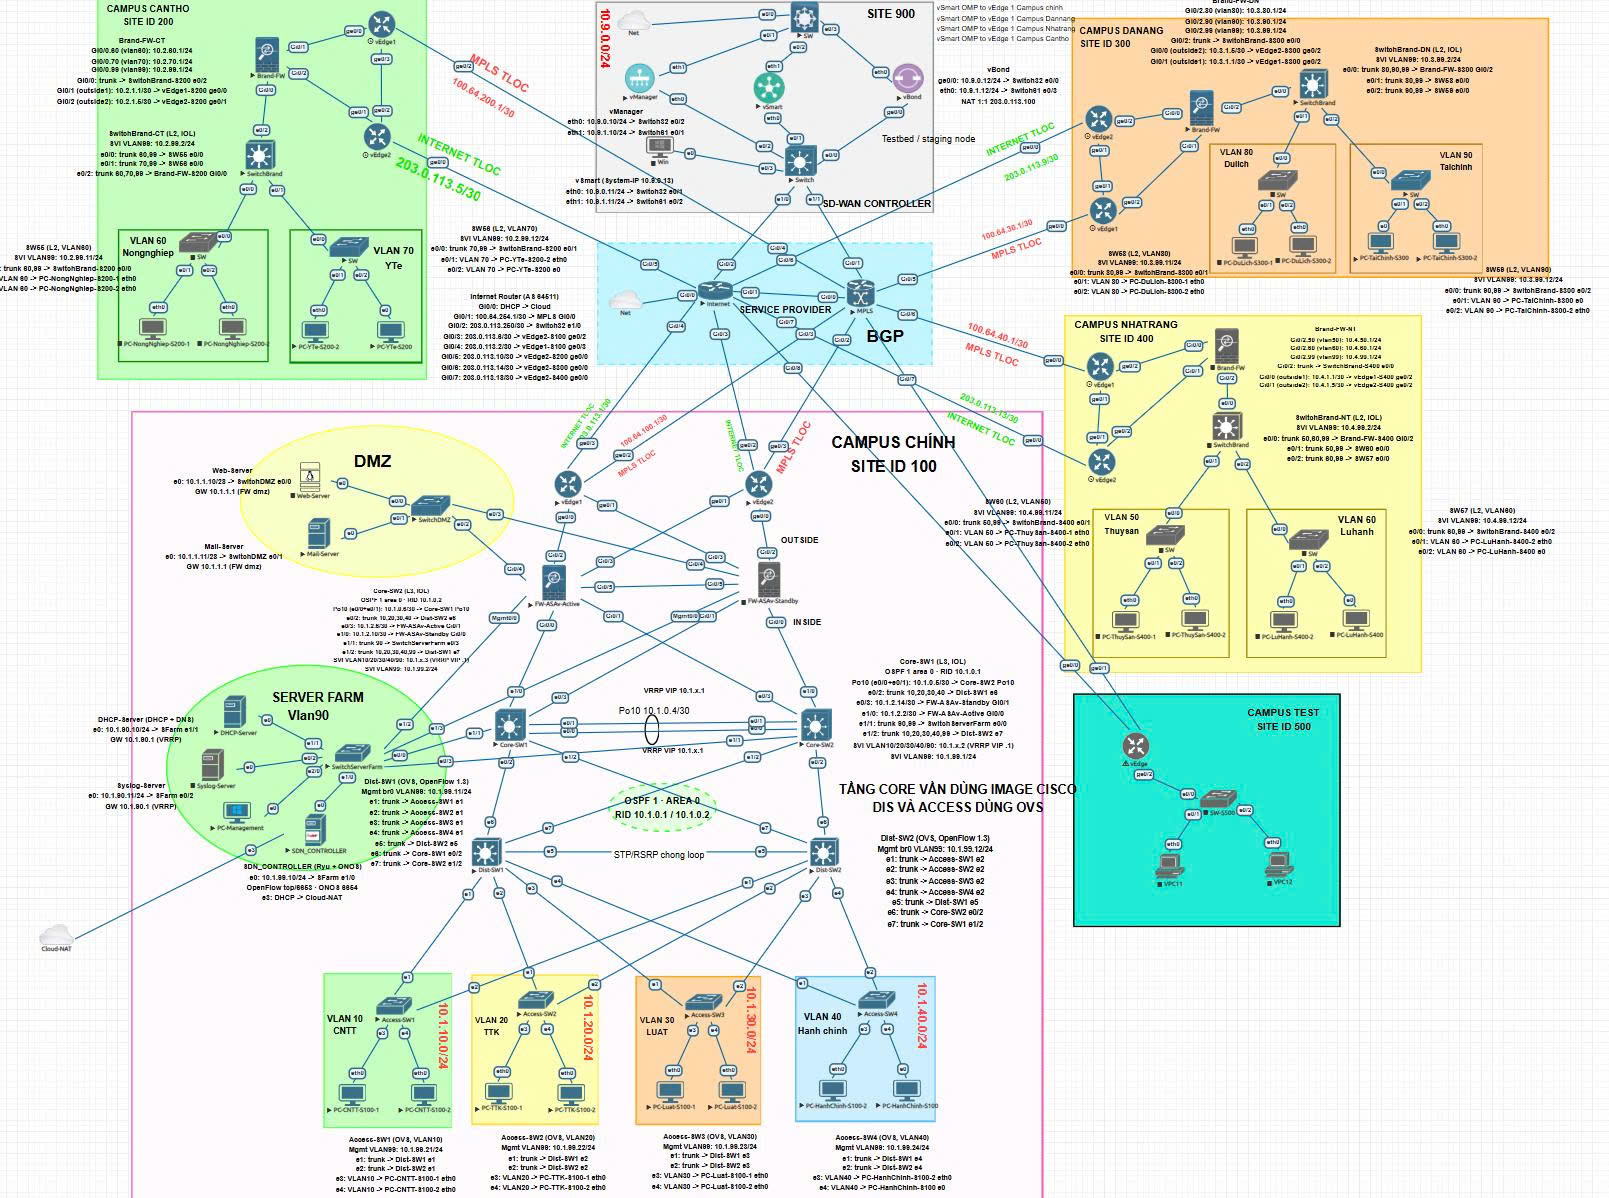
\includegraphics[height=0.78\textheight]{topo_tongthe.jpg}

    \scriptsize Campus chính Site 100 (SDN + FW-ASAv HA), chi nhánh 200/300/400, Site 500 (mở rộng),
    Site 900 (SD-WAN controller), nhà cung cấp Internet/MPLS chạy BGP -- 70 node, 103 network.
\end{frame}

\begin{frame}{Mục tiêu của tuần (26/10 -- 01/11) và mức độ hoàn thành}
    \centering
    \small
    \begin{tabular}{@{}p{0.70\textwidth}c@{}}
        \toprule
        \textbf{Nhiệm vụ đặt ra tuần trước} & \textbf{Trạng thái} \\
        \midrule
        Đo lặp SD-WAN: failover link WAN, khôi phục controller, độ sẵn sàng & \partly \\
        Kiểm thử failover cặp FW-ASAv HA và VRRP trên Core & \todo \\
        Hoàn thiện Site 500 (vEdge, switch, máy trạm, chính sách) & \done \\
        SDN: fast-failover cho uplink Distribution & \todo \\
        Theo dõi, thu bằng chứng khi vEdge mất kết nối & \done \\
        Đưa số liệu vào bản nháp báo cáo cuối kỳ & \todo \\
        \midrule
        \multicolumn{2}{@{}p{0.86\textwidth}@{}}{\textbf{Phát sinh thêm trong tuần:} kiểm thử tích hợp toàn hệ thống 70 node; sửa 2 lỗi làm mất Internet; \textbf{Campus NetOps Bot} (Telegram + AI agent) chạy thật, quản trị in-band Site 100 và 3 chi nhánh.} \\
        \bottomrule
    \end{tabular}
\end{frame}

% ============================================================
% PROGRESS
% ============================================================
\section{Kết quả thực hiện trong tuần}

\begin{frame}{Tổng quan tiến độ theo hạng mục}
    \centering
    \small
    \begin{tabular}{@{}llc@{}}
        \toprule
        \textbf{Giai đoạn} & \textbf{Hạng mục} & \textbf{Trạng thái} \\
        \midrule
        Khảo sát \& thiết kế    & Lý thuyết SDN/SD-WAN, topo, bảng IP/VLAN/ASN   & \done \\
        Hạ tầng campus L2/L3    & Core/Dist/Access, VRRP, FW-ASAv HA, ASDM       & \done \\
        Chi nhánh 200/300/400   & Brand-FW, DHCP, SwitchBrand, VPC              & \done \\
        SD-WAN                  & Controllers, PKI, vEdge, BFD, chính sách vSmart & \done \\
        SDN campus chính        & Ryu, Console, 5 mục tiêu, fast-failover        & \done \\
        Site 500                & 2 vEdge, Brand-FW, SW-S500, máy trạm nhận DHCP & \done \\
        Kiểm thử tích hợp       & Chức năng toàn hệ thống ĐẠT; còn kịch bản sự cố & \doing \\
        \textbf{NetOps Bot (mới)} & Telegram + AI agent, quản trị in-band        & \doing \\
        Báo cáo \& demo         & Báo cáo tuần, bảng tiến độ; báo cáo cuối kỳ, slide bảo vệ & \doing \\
        \bottomrule
    \end{tabular}
\end{frame}

\begin{frame}{SD-WAN -- Trạng thái fabric trên vManage (31/10)}
    \centering
    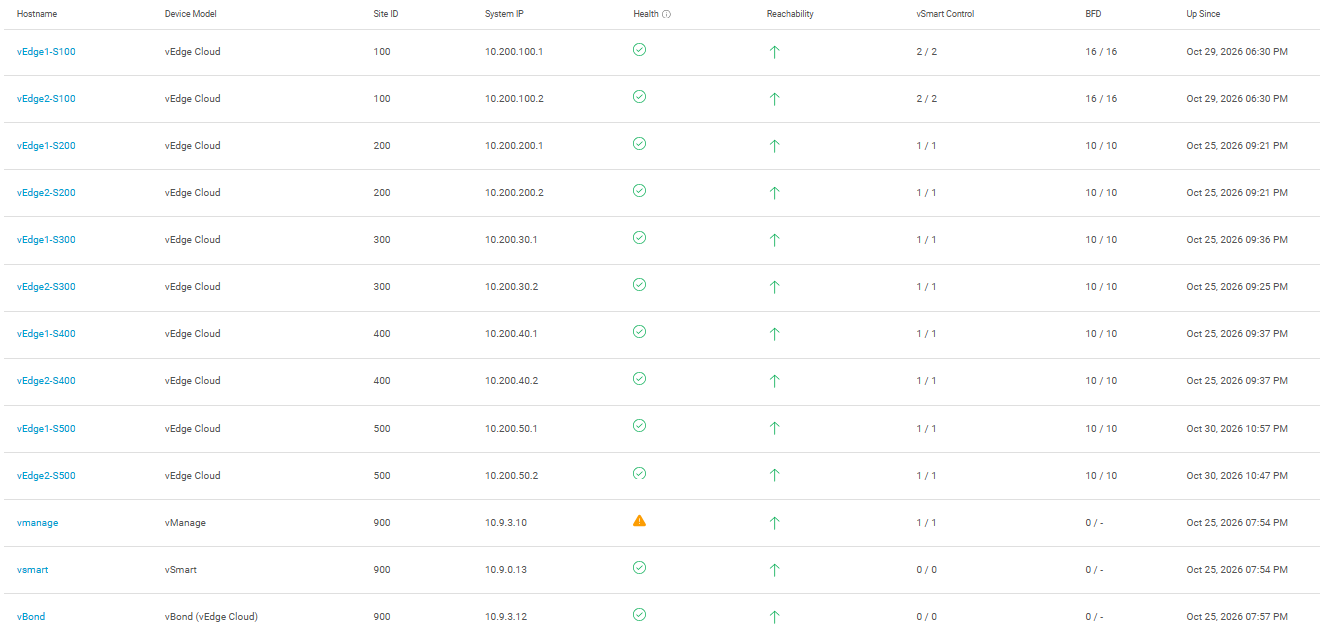
\includegraphics[height=0.74\textheight]{vmanage_devices.png}

    \vspace{0.15cm}
    \footnotesize \textbf{10/10 vEdge} (gồm \textbf{2 vEdge Site 500}) và 3 controller đều reachable, \textcolor{doneGreen}{\textbf{BFD đủ}} trên mọi vEdge
    (Site 100: 16/16, chi nhánh: 10/10).
\end{frame}

\begin{frame}{SD-WAN -- Các tunnel IPsec giữa các site}
    \centering
    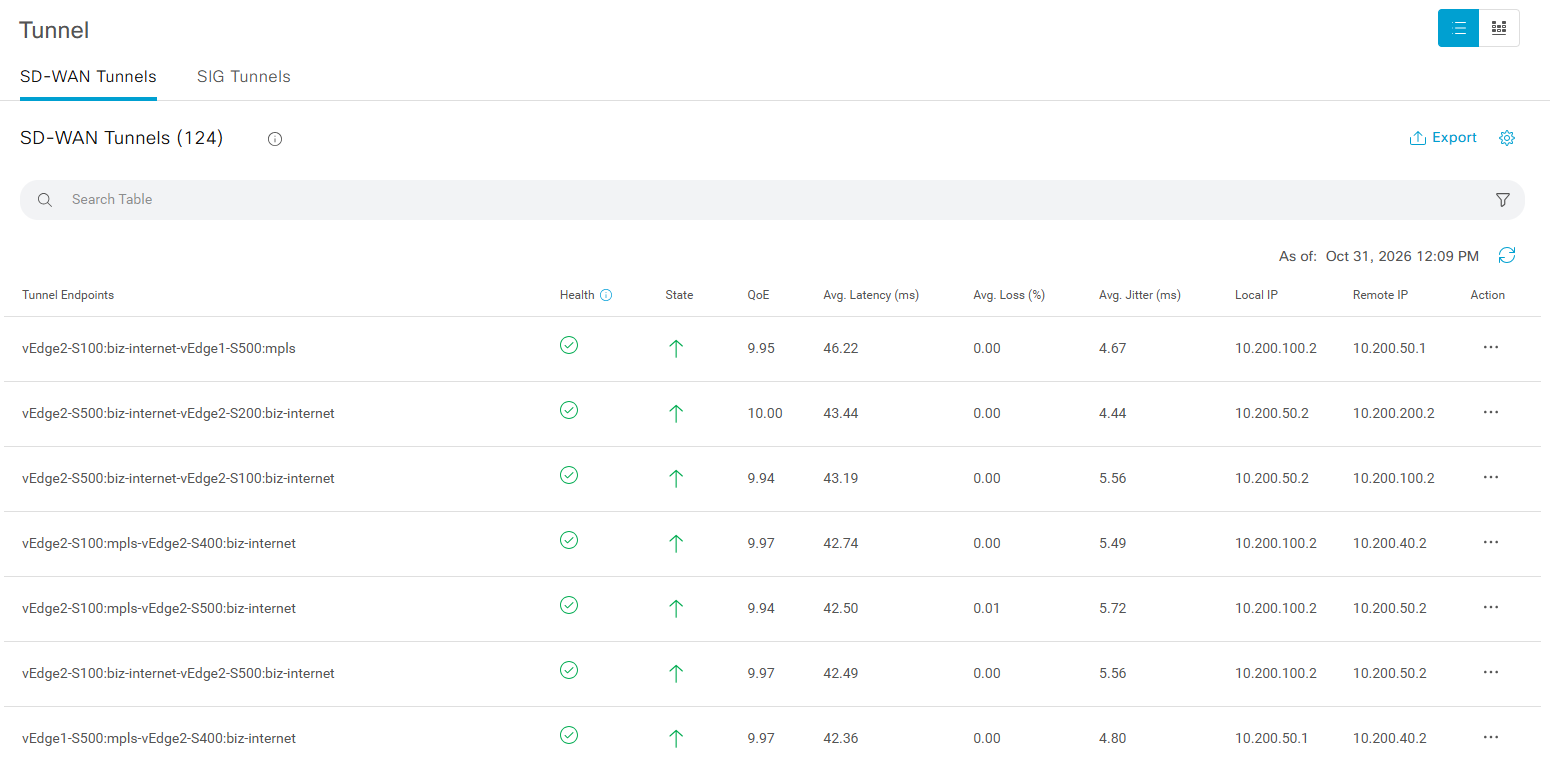
\includegraphics[height=0.76\textheight]{vmanage_tunnels.png}

    \vspace{0.1cm}
    \footnotesize 124 tunnel SD-WAN qua 2 màu \texttt{biz-internet} và \texttt{mpls}, gồm cả tunnel tới Site 500; mất gói trung bình $\approx$ 0\,\%.
\end{frame}

\begin{frame}{SD-WAN -- Đo failover link WAN tại Site 200 (24/10)}
    \begin{columns}[T]
        \begin{column}{0.58\textwidth}
            \centering
            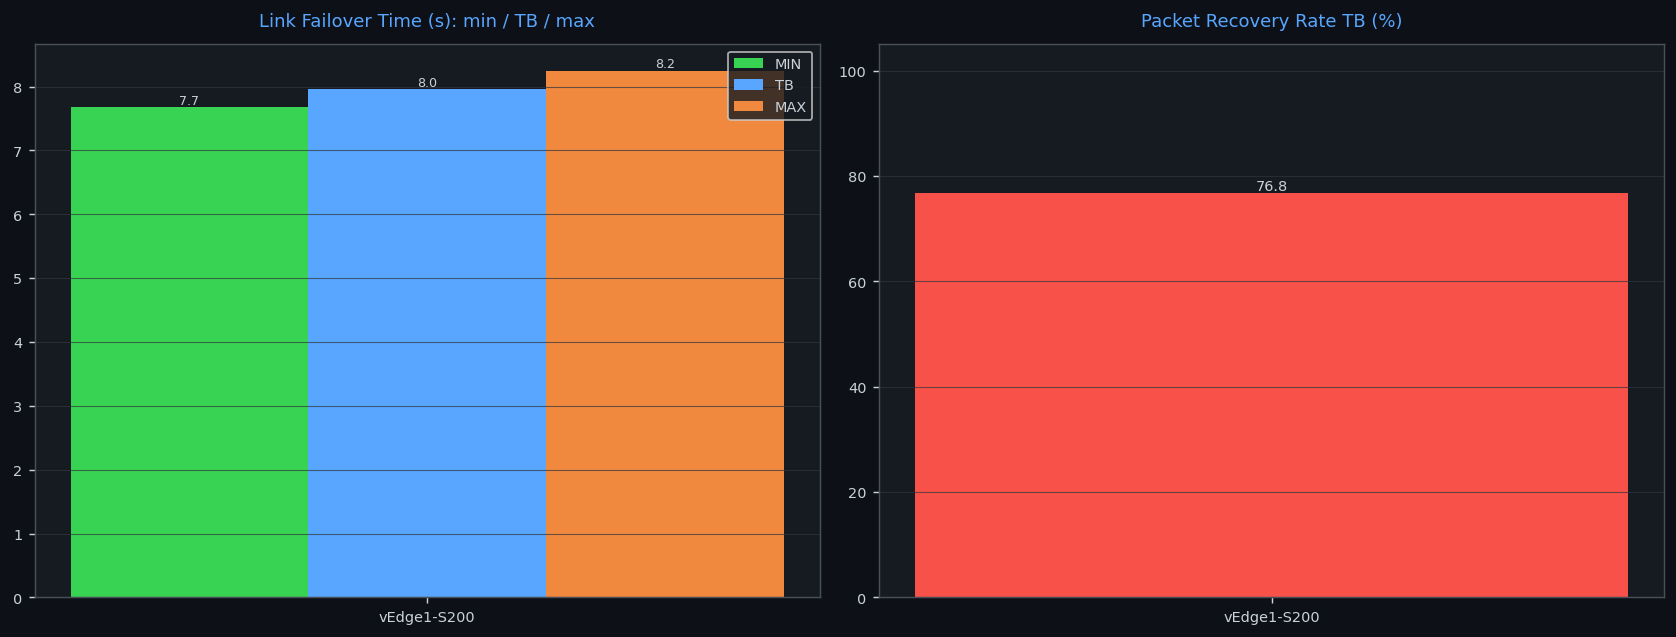
\includegraphics[width=\textwidth]{tincay_failover.png}

            \scriptsize Công cụ web tại Site 900: ping liên tục qua overlay trong lúc cắt uplink vEdge 1 Site 200.
        \end{column}
        \begin{column}{0.42\textwidth}
            \begin{block}{Kết quả (2 lần đo)}
                \small
                \begin{itemize}
                    \item RTO: \textbf{7,68 -- 8,25\,s}, trung bình \textbf{7,96\,s}.
                    \item Tỉ lệ khôi phục gói (PRR): \textbf{76,75\,\%}.
                \end{itemize}
            \end{block}
            \begin{alertblock}{Nhận xét}
                \small
                \begin{itemize}
                    \item $\approx$ 8\,s khớp BFD mặc định (hello 1\,s $\times$ 7).
                    \item Chậm hơn nhiều so với SDN fast-failover ($<$ 0,3\,s).
                    \item Mới 2 lần $\Rightarrow$ tuần tới đo đủ 3--5 lần, thử BFD ngắn hơn.
                \end{itemize}
            \end{alertblock}
        \end{column}
    \end{columns}
\end{frame}

\begin{frame}{SD-WAN -- So sánh hiệu năng Campus chính và chi nhánh (25/10)}
    \begin{columns}[T]
        \begin{column}{0.55\textwidth}
            \centering
            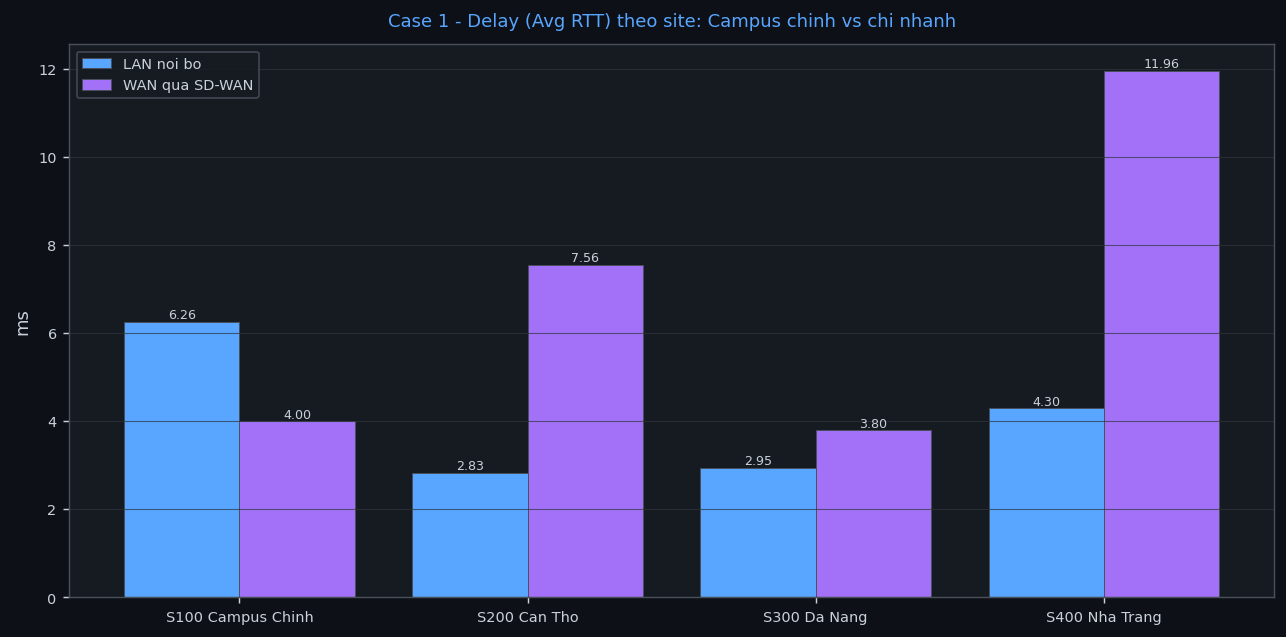
\includegraphics[width=\textwidth]{sosanh_delay.png}

            \scriptsize Delay trung bình: LAN nội bộ site và WAN qua SD-WAN.
        \end{column}
        \begin{column}{0.45\textwidth}
            \centering
            \footnotesize
            \begin{tabular}{@{}lccc@{}}
                \toprule
                \textbf{Site} & \textbf{Delay WAN} & \textbf{Jitter WAN} & \textbf{Mất gói} \\
                \midrule
                100 & 4,0\,ms  & 0,5\,ms  & 0\,\% \\
                200 & 7,6\,ms  & 5,1\,ms  & 0\,\% \\
                300 & 3,8\,ms  & 0,4\,ms  & 0\,\% \\
                400 & 12,0\,ms & 10,3\,ms & 0\,\% \\
                \bottomrule
            \end{tabular}
            \vspace{0.2cm}

            \begin{block}{Nhận xét}
                \scriptsize
                \begin{itemize}
                    \item WAN qua SD-WAN \textbf{không mất gói} ở cả 4 site.
                    \item Site 400 jitter cao do vài mẫu RTT vọt 25--50\,ms $\Rightarrow$ cần đo lặp.
                    \item Site 100 chỉ đo được 3/5 tuyến LAN: FW chặn ICMP vào Server Farm/DMZ
                          (đúng chính sách) $\Rightarrow$ đổi cách đo.
                \end{itemize}
            \end{block}
        \end{column}
    \end{columns}
\end{frame}

\begin{frame}{Kiểm thử tích hợp toàn hệ thống (bật đủ 70 node)}
    \centering
    \small
    \begin{tabular}{@{}p{0.22\textwidth}p{0.58\textwidth}c@{}}
        \toprule
        \textbf{Cụm} & \textbf{Kết quả} & \textbf{Đánh giá} \\
        \midrule
        SDN Site 100      & 6/6 OVS, 13/13 liên kết; 7/7 máy trạm nhận DHCP, thông liên VLAN & \done \\
        Firewall HA       & FW-ASAv Active / Standby Ready & \done \\
        SD-WAN            & 12/12 thiết bị reachable, BFD 92/92 & \done \\
        Chi nhánh         & 9/9 VPC + 3 PC Linux nhận DHCP; tới Web/Mail/DNS Site 100 (TCP 80, 443, 25, 143, 587) & \done \\
        Internet          & 4/4 site ra Internet (sau khi sửa lỗi Site 500) & \done \\
        Quản trị in-band  & Từ Site 100 ping 15/15 IP quản trị chi nhánh; SSH 12/12 thiết bị & \done \\
        \bottomrule
    \end{tabular}
    \vspace{0.3cm}

    \footnotesize Đã đạt toàn bộ kiểm thử \textbf{chức năng}; tuần tới chuyển sang kiểm thử \textbf{sự cố} (failover FW, cắt 1 màu WAN).
\end{frame}

\begin{frame}{Hai lỗi định tuyến làm mất Internet đã sửa}
    \begin{columns}[T]
        \begin{column}{0.5\textwidth}
            \begin{block}{Mọi site mất Internet khi Site 500 lên fabric}
                \small
                \begin{itemize}
                    \item Router Internet nhận \textbf{default route} từ vEdge Site 500 qua BGP
                          $\Rightarrow$ đường ra Internet của các site bị kéo sai hướng.
                    \item Sửa: bộ lọc BGP chặn default route đi vào từ neighbor Site 500.
                    \item Kết quả: 4/4 site ra Internet lại, Site 500 vẫn trong fabric.
                \end{itemize}
            \end{block}
        \end{column}
        \begin{column}{0.5\textwidth}
            \begin{block}{Site 100 mất Internet (chiều về bị drop)}
                \small
                \begin{itemize}
                    \item Core-SW1 và Core-SW2 quảng bá OSPF cùng cost; ASA \textbf{không chia tải qua 2 interface khác nhau}
                          $\Rightarrow$ gói chiều về vào sai interface bị drop.
                    \item Sửa: \texttt{ip ospf cost 10} trên các SVI của Core-SW2; SwitchServerFarm dùng default route.
                    \item Kết quả: máy trạm Site 100 ra Internet bình thường.
                \end{itemize}
            \end{block}
        \end{column}
    \end{columns}
\end{frame}

\begin{frame}{Campus NetOps Bot -- Kiến trúc in-band}
    \begin{columns}[T]
        \begin{column}{0.55\textwidth}
            \centering
            \begin{tikzpicture}[
                box/.style={draw=primaryDark, fill=lightGrayBg, rounded corners=2pt, align=center,
                            font=\scriptsize, minimum height=0.75cm, text width=2.3cm},
                bot/.style={box, fill=primaryDark!12, text width=3.0cm, minimum height=1.1cm},
                arr/.style={-{Stealth[length=4pt]}, thick, accentTeal}]
                \node[box] (tg) {Quản trị viên\\Telegram};
                \node[bot, below=0.45cm of tg] (bot) {\textbf{NetOps Bot}\\LangGraph + LLM\\(DHCP-Server Site 100)};
                \node[box, below left=0.6cm and -0.9cm of bot] (s100) {Site 100\\Core, FW-ASAv\\(SSH in-band)};
                \node[box, below right=0.6cm and -0.9cm of bot] (br) {Chi nhánh 200/300/400\\Brand-FW, switch\\(SSH qua SD-WAN)};
                \node[box, left=0.35cm of bot, text width=1.6cm] (vm) {vManage\\REST API};
                \node[box, right=0.35cm of bot, text width=1.6cm] (ryu) {Ryu\\REST API};
                \draw[arr, <->] (tg) -- (bot);
                \draw[arr] (bot) -- (s100);
                \draw[arr] (bot) -- (br);
                \draw[arr] (bot) -- (vm);
                \draw[arr] (bot) -- (ryu);
            \end{tikzpicture}
        \end{column}
        \begin{column}{0.45\textwidth}
            \begin{block}{Ý tưởng}
                \small
                \begin{itemize}
                    \item Bot cài \textbf{ngay trong topology}: là một ``người dùng'' của mạng, mạng hỏng thì bot biết đầu tiên.
                    \item Hỏi bằng lệnh hoặc \textbf{ngôn ngữ tự nhiên}; AI agent tự chọn công cụ (SSH, REST, DHCP).
                \end{itemize}
            \end{block}
            \begin{exampleblock}{Rào an toàn}
                \small
                \begin{itemize}
                    \item Chỉ trả lời chat được cho phép; mặc định chỉ lệnh đọc.
                    \item Che mật khẩu/khóa trong kết quả.
                    \item Tài khoản \texttt{netops} riêng, thiết bị chỉ nhận SSH từ 2 IP quản trị.
                \end{itemize}
            \end{exampleblock}
        \end{column}
    \end{columns}
\end{frame}

\begin{frame}{Campus NetOps Bot -- Ba giai đoạn đã triển khai}
    \begin{columns}[T]
        \begin{column}{0.33\textwidth}
            \begin{block}{GĐ1 -- Chỉ đọc}
                \small
                \begin{itemize}
                    \item Danh mục 47 thiết bị khớp topology.
                    \item \texttt{/show}, \texttt{/health}.
                    \item Hỏi đáp tự nhiên qua AI agent.
                \end{itemize}
            \end{block}
        \end{column}
        \begin{column}{0.33\textwidth}
            \begin{block}{GĐ2 -- Chẩn đoán}
                \small
                \begin{itemize}
                    \item Tự báo Telegram khi vEdge mất kết nối, OVS rời controller.
                    \item \texttt{/diag} \textbf{theo lớp}, dừng ở lớp đầu tiên sai: vEdge (6 lớp), FW, DHCP, chi nhánh.
                \end{itemize}
            \end{block}
        \end{column}
        \begin{column}{0.33\textwidth}
            \begin{block}{GĐ3 -- Thay đổi}
                \small
                \begin{itemize}
                    \item \texttt{/change}: duyệt trên Telegram rồi mới áp, \textbf{tự rollback} nếu mất kết nối.
                    \item \texttt{/compliance}, \texttt{/backup}, \texttt{/drift}.
                \end{itemize}
            \end{block}
        \end{column}
    \end{columns}
    \vspace{0.3cm}

    \begin{exampleblock}{Ví dụ: \texttt{/diag site 400}}
        \small
        vEdge $\rightarrow$ WAN Brand-FW $\rightarrow$ gateway $\rightarrow$ trunk $\rightarrow$ DHCP.
        Bot phát hiện \textbf{lệch thiết kế có thật}: uplink 2 switch phòng ban Site 400 lên trunk nhờ DTP tự thỏa thuận,
        không cấu hình tường minh $\Rightarrow$ giữ lại làm kịch bản demo sửa bằng \texttt{/change}.
    \end{exampleblock}
\end{frame}

\begin{frame}{Campus NetOps Bot -- Mở rộng ra chi nhánh \& kiểm thử}
    \begin{columns}[T]
        \begin{column}{0.5\textwidth}
            \begin{block}{Quản trị chi nhánh qua overlay SD-WAN}
                \small
                \begin{itemize}
                    \item 12 thiết bị (Brand-FW, SwitchBrand, 2 switch phòng ban $\times$ 3 site).
                    \item Switch: user \texttt{netops}, SSH v2, ACL chỉ cho 2 IP quản trị, default route về Brand-FW.
                    \item Brand-FW: AAA LOCAL + tự vào chế độ đặc quyền; SSH chỉ từ 2 IP quản trị.
                    \item Cấu hình lưu trên thiết bị và đồng bộ về kho mã nguồn.
                \end{itemize}
            \end{block}
        \end{column}
        \begin{column}{0.5\textwidth}
            \begin{exampleblock}{Kết quả kiểm thử}
                \small
                \begin{itemize}
                    \item Ping \textbf{15/15} IP quản trị chi nhánh từ Site 100.
                    \item Selftest trên DHCP-Server: \textbf{23/23 ĐẠT}.
                    \item \textbf{71} unit test + kiểm cú pháp toàn bộ mã nguồn.
                    \item Chẩn đoán vEdge qua vManage: \textbf{8/8 vEdge đạt cả 6 lớp}.
                    \item Lệnh và câu hỏi tự nhiên trên Telegram chạy thật.
                \end{itemize}
            \end{exampleblock}
        \end{column}
    \end{columns}
\end{frame}

% ============================================================
% UNFINISHED
% ============================================================
\section{Công việc chưa hoàn thành}

\begin{frame}{Vấn đề còn tồn tại}
    \begin{alertblock}{Chưa xử lý xong}
        \begin{itemize}
            \item \textbf{Kiểm thử sự cố:} chưa failover cặp FW-ASAv HA, VRRP; chưa cắt 1 màu WAN để xem BFD/AAR chuyển đường.
            \item \textbf{Đo lặp SD-WAN:} failover link WAN mới 2 lần tại 1 site; chưa đo khôi phục khi mất vSmart.
            \item \textbf{Site 500:} LAN đã xong; chưa kiểm thử tích hợp (Web/Mail/DNS, Internet) như 3 chi nhánh.
            \item \textbf{SDN:} mất liên kết Distribution -- Core vẫn gián đoạn 2--3,7\,s (chưa có fast-failover).
            \item \textbf{NetOps Bot:} chưa có rollback cho ASA; trunk Site 400 chưa sửa (để demo).
            \item \textbf{Báo cáo cuối kỳ:} chưa bắt đầu bản nháp.
        \end{itemize}
    \end{alertblock}
\end{frame}

% ============================================================
% NEXT WEEK
% ============================================================
\section{Kế hoạch tuần tới}

\begin{frame}{Nhiệm vụ tuần tới (02/11 -- 08/11/2026)}
    \begin{columns}[T]
        \begin{column}{0.5\textwidth}
            \begin{block}{Kỹ thuật}
                \small
                \begin{enumerate}
                    \item Failover cặp FW-ASAv HA và VRRP Core-SW1/2: số gói mất, thời gian chuyển và quay về.
                    \item Cắt 1 màu WAN xem BFD/AAR chuyển đường; đo lặp failover 3--5 lần/site; đo khôi phục khi mất vSmart.
                    \item Site 500: kiểm thử tích hợp như 3 chi nhánh; đưa vào NetOps Bot.
                    \item SDN: thử fast-failover cho uplink Distribution -- Core (nếu kịp).
                \end{enumerate}
            \end{block}
        \end{column}
        \begin{column}{0.5\textwidth}
            \begin{block}{NetOps \& báo cáo}
                \small
                \begin{enumerate}
                    \setcounter{enumi}{4}
                    \item NetOps Bot: rollback cho ASA; kịch bản demo ``phát hiện -- sửa trunk Site 400 bằng \texttt{/change} -- tự rollback''.
                    \item Đo lại tuyến LAN Site 100 theo cách mới; theo dõi độ sẵn sàng nhiều ngày.
                    \item Bắt đầu báo cáo cuối kỳ: chương kết quả (SDN, SD-WAN, tích hợp) và chương NetOps Bot.
                \end{enumerate}
            \end{block}
        \end{column}
    \end{columns}
    \vspace{0.2cm}
    \centering\footnotesize Hạn kiểm thử tích hợp: \textbf{10/11/2026}. Đo SDN và SD-WAN không chạy đồng thời để tránh nhiễu.
\end{frame}

% ============================================================
% DIFFICULTIES
% ============================================================
\section{Khó khăn}

\begin{frame}{Khó khăn gặp phải trong tuần}
    \small
    \begin{itemize}
        \item \textbf{Lỗi chỉ lộ ra khi bật toàn hệ thống:} Site 500 lên fabric làm \emph{mọi} site mất Internet --
              phải lần theo BGP trên router Internet mới thấy default route đi sai hướng.
        \item \textbf{Hành vi riêng của ASA:} không chia tải qua 2 interface khác nhau; tài khoản mới bị bắt đổi mật khẩu
              ở lần SSH đầu (đăng nhập console không xóa được cờ này); cấm mật khẩu có chuỗi ký tự liên tiếp.
        \item \textbf{SSH cũ trên IOL:} client chỉ hỗ trợ SHA-1, phải tạm nới thuật toán trên ASA rồi trả lại.
        \item \textbf{LLM miễn phí bị giới hạn tần suất (HTTP 429):} chuyển sang API chuẩn OpenAI, thêm thử lại
              và model dự phòng; đổi nhà cung cấp chỉ cần sửa file cấu hình.
        \item \textbf{Triển khai trên Windows Server 2012 R2:} hệ điều hành cũ,
              phải đóng gói bộ cài offline (Python 3.11 + thư viện); một lỗi cú pháp khi chép mã làm bot khởi động lại liên tục
              $\Rightarrow$ thêm test kiểm cú pháp trước khi triển khai.
        \item \textbf{Đo hiệu năng:} chính sách firewall chặn ICMP làm sai số đo tuyến LAN Site 100.
    \end{itemize}
\end{frame}

\begin{frame}[plain]
    \centering
    \vfill
    {\Huge\color{primaryDark}\textbf{Cảm ơn thầy đã lắng nghe!}}
    \vfill
\end{frame}

\end{document}
